%! LuaLaTeX 文書
\usetheme{metropolis}
\usefonttheme{professionalfonts}

\hypersetup{linkcolor=,urlcolor=teal}

\usepackage{luatexja}
\ltjsetparameter{jacharrange={-2,-3,-8}}
\usepackage[no-math,match,deluxe]{luatexja-preset}

\usepackage{textcomp}
\usepackage{luatexja-otf}

\usepackage{graphicx,xcolor}
\usepackage{pxrubrica}
\usepackage{tcolorbox}
\usepackage{bxwareki}
\usepackage{indentfirst}

\usepackage{listings}
\lstset{
	doubleletterspace,
	basicstyle={\small\ttfamily},
	backgroundcolor={\color[gray]{.9}},
	commentstyle={\color[gray]{.5}},
	numbers=left,
	numberstyle=\tiny,
}

\usepackage{tikz}
\usetikzlibrary{plotmarks}

\usepackage{scsnowman} %☃
\usepackage{bxokumacro}
\usepackage{menukeys}
\renewmenumacro{\keys}{shadowedroundedkeys}
\usepackage{bxrawstr} % https://zrbabbler.hatenablog.com/entry/20181222/1545495849
\usepackage[twemoji-pdf]{bxcoloremoji} % https://github.com/zr-tex8r/BXcoloremoji

\usepackage{mflogo}

\usepackage{bxtexlogo}
\bxtexlogoimport{*,**}

\usepackage[T1]{fontenc}
\usepackage{mathtools,amssymb,mathrsfs,mathabx}
\usepackage[math]{iwona}
\usepackage[euler-digits]{eulervm}
\allowdisplaybreaks[4]

%%%%%%%%%% 商用フォントを用いているので、自分でタイプセットする場合は適当に以下を変えてください
\setmainfont[
	Ligatures=TeX,
	BoldFont=FOT-RodinNTLGPro-EB,
	ItalicFont=FOT-RodinNTLGPro-EB,
]{FOT-RodinNTLGPro-B}
\setsansfont[
	Ligatures=TeX,
	BoldFont=FOT-RodinNTLGPro-EB,
	ItalicFont=FOT-RodinNTLGPro-EB,
]{FOT-RodinNTLGPro-B}
\setmainjfont[
	Ligatures=TeX,
	CharacterWidth=Proportional,
	JFM=prop,
	BoldFont=FOT-RodinNTLGPro-EB,
	ItalicFont=FOT-RodinNTLGPro-EB,
]{FOT-RodinNTLGPro-B}
\setsansjfont[
	Ligatures=TeX,
	CharacterWidth=Proportional,
	JFM=prop,
	BoldFont=FOT-RodinNTLGPro-EB,
	ItalicFont=FOT-RodinNTLGPro-EB,
]{FOT-RodinNTLGPro-B}
\setmonofont[
	Ligatures=TeXReset,
]{HackGen}
\setmonojfont[
	Ligatures=TeXReset,
]{HackGen}

\newfontfamily\errorfont[
	Ligatures=TeX,
]{TsukuQMinLStd-L}

\newfontfamily\nishikifonta[
	Ligatures=TeX,
]{Nishiki-teki}
\newjfontfamily\nishikifontj[
	Ligatures=TeX,
]{Nishiki-teki}
\newcommand{\nishikifont}{\nishikifonta\nishikifontj}

%%%%%%%%%% 以下は自前コマンド

\newcommand{\centeralign}[1]{\rule{0pt}{0pt}\hfill#1\hfill\rule{0pt}{0pt}}
\newcommand{\typecommand}[1]{\colorbox{darkgray}{{\ttfamily\color{lime}#1}}}
\newcommand{\typecmdbox}[1]{
	\begin{tcolorbox}[
		sharp corners,left=0mm,right=0mm,top=0mm,bottom=0mm,
		colframe=darkgray,
		colback=darkgray,
	]
		{\ttfamily\color{lime}#1}
	\end{tcolorbox}
}

\setlength{\parskip}{2ex}

\title{最大限 \TeX 入門}
\subtitle{インストールと利用法}
\author{北海道大学理学部 ひとみさん}
\date{\warekitoday}

\begin{document}
\rubyusejghost % \jruby で和文ゴースト

\frame{\maketitle}

\begin{frame}
	\frametitle{参考文献}
	\begin{columns}[c]
		\begin{column}{0.7\textwidth}
			[改訂第 7 版] \LaTeXe 美文書作成入門
			{\small (奥村晴彦・黒木祐介 著 技術評論社\textbf{(2017)})}
			
			\begin{itemize}
				\item 3年毎に改版\\(2020 年に改版)
				\item 「とりあえずこれを読め」
			\end{itemize}
		\end{column}
		\begin{column}{0.25\textwidth}
			\fbox{
\includegraphics[width=\textwidth]{bibunsho.jpg}}
		\end{column}
	\end{columns}
	{\nishikifont 😀 美文書何章に記述があるか適宜参照します 😀}
\end{frame}

\begin{frame}
	\frametitle{扱うことと扱わないこと}
	\begin{block}{扱うこと}
		\begin{itemize}
			\item \TeX とはなにか
			\item \TeX のインストール方法
			\item \TeX の初歩的な使い方
		\end{itemize}
	\end{block}
	\begin{block}{扱わないこと}
		\begin{itemize}
		\item 文書を書くのに使う\jruby[g]{命令}{コマンド}
			{\nishikifont\small (美文書 3, 5--11 章の大半)}
		\item \jruby[g]{命令}{コマンド}の作成
			{\nishikifont\small (美文書 4 章)}
		\item \coloremoji{🍣}\TeX 言語 \coloremoji{🤮}
		\end{itemize}
	\end{block}
\end{frame}

\begin{frame}
	\frametitle{目次}
	\setlength{\parskip}{0.5ex}
	\tableofcontents
\end{frame}

\frame{\section{\TeX 概観}{\nishikifont 😀 美文書 1 章 😀}}

\begin{frame}
	\frametitle{\protect\TeX でできること、特徴}
	文字を並べた PDF を作ることができる。
	\pause
	\begin{itemize}
		\item きれいな数式
			\[\int_0^\infty \frac{\sin x}{\sqrt{x}}\,dx
			=\sum_{k=0}^\infty \frac{(2k)!}{2^{2k (k!)^2}}\frac{1}{2k+1}=\frac{\pi}{2}\]
		\item 相互参照、処理の自動化
		\item フリーソフト
		\item 様々な OS で利用可能
		\item 実体はテキストファイル
	\end{itemize}
\end{frame}

\begin{frame}
	\frametitle{\TeX でできないこと}
	\begin{itemize}
		\item 見たまま編集\\
			{\footnotesize Word などを使えば良い、もしくは\LyX?}
		\item 図の描画\\
			{\footnotesize ほかソフトで作ってから埋め込めば良い、もしくは\TikZ?}
		\item フォントを自在に扱う\\
			{\footnotesize \LuaTeX や \XeTeX で使える fontspec パッケージを使えば……}
	\end{itemize}
\end{frame}

\begin{frame}
	\frametitle{\TeX とは何か}
	\begin{itemize}
		\item 1978 年に Donald E. Knuth が発表
			\begin{itemize}
				\item 相当に古い
			\end{itemize}
		\item 組版システム
			\begin{itemize}
				\item 組版するための\emph{ソフトウェア}
				\item 組版するための\emph{プログラミング言語}
			\end{itemize}
			\pause
		\item \LaTeX
			\begin{itemize}
				\item \TeX とは別物
				\item \TeX のマクロ体系(フォーマット)
			\end{itemize}
	\end{itemize}
\end{frame}

\begin{frame}
	\frametitle{ナントカ\TeX}
	\TeX の仲間にはたくさんある(ナントカ\TeX )
	\begin{itemize}
		\item 処理系……\TeX (ソフトウェア)を拡張したもの\\
			{\eTeX}, {\pdfTeX}, {\XeTeX}, {\LuaTeX}, {\pTeX}, {\upTeX} など
		\item フォーマット……マクロ体系\\
			{\LaTeX}, {plain \TeX}, {\ConTeXt} など
	\end{itemize}
	全部まとめて\TeX と呼ぶことも多い
\end{frame}

\begin{frame}
	\frametitle{\TeX ディストリビューション}
	\TeX に関する成果物は、CTAN に集められる
	\begin{itemize}
		\item \url{https://www.ctan.org}
		\item ボランティアで成り立っている
	\end{itemize}
	
	CTAN から様々なディストリビューション(配布元)へ
	\begin{itemize}
		\item {\TeX} Live (\url{http://www.tug.org/texlive/})
		\item W32TeX (\url{http://w32tex.org/})\footnote{{\TeX} Live がベース}
		\item MiK{\TeX} (\url{https://miktex.org})\footnote{日本語できない模様}
	\end{itemize}
\end{frame}

\begin{frame}
	\frametitle{\TeX ディストリビューション}
	\TeX 本体やパッケージ以外にも、関連するバイナリも収録されている
	
	\begin{itemize}
		\item dvi ウェア(後述)
		\item kpathsea(後述)
		\item texdoc
	\end{itemize}
	
	texdoc → ドキュメントを検索するコマンド\\
	{\footnotesize 例: \typecommand{texdoc latex}}
	
	\typecommand{\Large texdoc platexsheet-jsclasses}\\でコマンド一覧を表示\\
	{\footnotesize ワトソン氏(朝倉卓人)作成}
\end{frame}

\begin{frame}
	\frametitle{{\TeX} Live}
	最も普及している \TeX ディストリビューション
	
	膨大な数のパッケージやバイナリが含まれる
	
	晩春に名前が変わる大型アップデート\\
	{\footnotesize 2 月頃に更新停止 (frozen)・次年度版の pretest\\
	2020 年 4 月 10 日~{\TeX} Live 2019 → {\TeX} Live 2020}
	
	バイナリの更新は原則\emph{大型アップデート時のみ}\\
	{\footnotesize パッケージ(テキストファイル)の更新は frozen 時以外はいつでも}
	
	大型アップデート時はインストールし直す必要
\end{frame}

\frame{\section{\TeX のインストール} {\nishikifont 🖳 美文書 付録 A 🖳}}

\begin{frame}
	\frametitle{\TeX のインストール}
	Windows なら W32TeX\\
	それ以外なら {\TeX} Live をインストール
	
	詳しくは {\TeX} Wiki\footnote{\url{https://texwiki.texjp.org}}\\
	または \url{http://www.circle9.work/tex/install.html}
	
	インストールには数時間かかります。
\end{frame}

\begin{frame}
	\frametitle{最新の {\TeX} Live をインストールする---UNIX 系の場合}
	TUG\footnote{{\TeX} User Group \url{ftp://ftp.tug.org/texlive/tlnet/}}
	からインストーラをダウンロード\footnote{ミラーサイトを利用しましょう}\\
	\typecommand{\scriptsize wget http://mirror.ctan.org/systems/texlive/tlnet/install-tl-unix.tar.gz}
	
	インストーラを起動してインストール\\
	\typecmdbox{\scriptsize sudo ./install-tl -no-gui \textbackslash\\
	~~~~-repository http://mirror.ctan.org/systems/texlive/tlnet}
	
	ネットワーク経由なので電波の良いところで
\end{frame}

\begin{frame}
	\frametitle{{\TeX} Live のアップデート}
	({\TeX} Live をインストールした場合)
	
	\centeralign{\typecommand{sudo tlmgr update --self --all}}
	
	上のコマンドで {\TeX} Live をアップデート
	
	定期的にやろう
	
	年度が変わる大型アップデート時には\emph{再インストール}
\end{frame}

\frame{\section{\TeX の使い方} {\nishikifont 😀 美文書 2 章 😀}}

\begin{frame}
	\frametitle{\TeX の使い方}
	自分で書いた \TeX ソースを、\TeX 処理系に処理させることで、PDF ファイルを得る。\par
	\pause
	\centeralign{\emph{のだが}}\par
	\pause
	歴史的経緯で、\TeX 処理系は、PDF ファイルではなく、\emph{dvi ファイル}を出力する
	\footnote{新しい処理系には、直接 PDF を出力するものもある。\\例: \pdfTeX, \LuaTeX, \XeTeX}。
	
	出てきた dvi ファイルを dvi ウェアで処理することによって、最終的な PDF を得ることができる。
\end{frame}

\begin{frame}
	\frametitle{PDF を得る流れ}
	\begin{columns}[c]
		\begin{column}{0.6\textwidth}
			\begin{description}
				\item[\TeX 処理系] 文字の座標を決める
				\item[dvi ウェア] 実際に文字を配置する
			\end{description}
		\end{column}
		\begin{column}{0.4\textwidth}
			\centering
			\begin{tikzpicture}
				\node[draw](tex)at(0,0){.tex ファイル};
				\node[draw](dvi)at(0,-2){.dvi ファイル};
				\node[draw](pdf)at(0,-4){.pdf ファイル};
				\draw[->,very thick](tex)--(dvi)--(pdf);
				\coordinate(A)at(0,-1);
				\coordinate(B)at(0,-3);
				\node[right](T)at(0.5,-1){\TeX 処理系};
				\node[right](D)at(0.5,-3){dvi ウェア};
				\draw[<-](A)--(T);\draw[<-](B)--(D);
			\end{tikzpicture}
		\end{column}
	\end{columns}
\end{frame}

\begin{frame}
	\frametitle{dvi ウェア}
	dvi ← \textbf{D}e\textbf{v}ice \textbf{I}ndependent (装置非依存)
	
	dvi ウェア……dvi ファイルを変換するソフトウェア
	
	\begin{itemize}
		\item dvipdfmx(PDF に変換)
		\item dvips(PostScript に変換)
	\end{itemize}
	
	\begin{block}{dvi の仕様}
		\begin{description}
			\item[標準仕様] 装置非依存な部分。dvi ウェアで共通。
			\item[拡張仕様] 装置依存な部分\footnote{色とか用紙サイズとか}。
				dvi ウェアごとに\emph{異なる}。
		\end{description}
	\end{block}
\end{frame}

\begin{frame}
	\frametitle{\TeX ソースを書くうえでの注意点}
	使う\TeX 処理系、dvi ウェアによって書き方が微妙に違う
	
	\emph{どの処理系、どの dvi ウェアを利用するか気に留める必要}
	
	\pause
	\begin{block}{日本で一般的な方法}
		\begin{itemize}
			\item {\pLaTeX} + dvipdfmx
			\item {\upLaTeX} + dvipdfmx
			\item {\LuaLaTeX}(最近広まりつつある)
		\end{itemize}
	\end{block}
	
	以下、主に {\pLaTeX} + dvipdfmx を例にして話す
	\footnote{\LuaLaTeX は (u)p\LaTeX と書き方がそれなりに異なるので注意}
\end{frame}

\frame{\section{\LaTeX の書き方}{\nishikifont 🤓美文書 3 章🤓}}

\begin{frame}[fragile]
	\frametitle{\LaTeX 文書の作り方}
	\lstinputlisting[caption={sample.tex}]{sample.tex}
	
	BOM なし UTF-8 で保存しましょう
\end{frame}

\begin{frame}
	\frametitle{\LaTeX 文書の作り方}
	\begin{columns}[c]
		\begin{column}{0.5\textwidth}
			コマンドラインで以下を実行
	
			\typecommand{platex sample}
	
			\typecommand{dvipdfmx sample}
		\end{column}
		\begin{column}{0.4\textwidth}
			\fbox{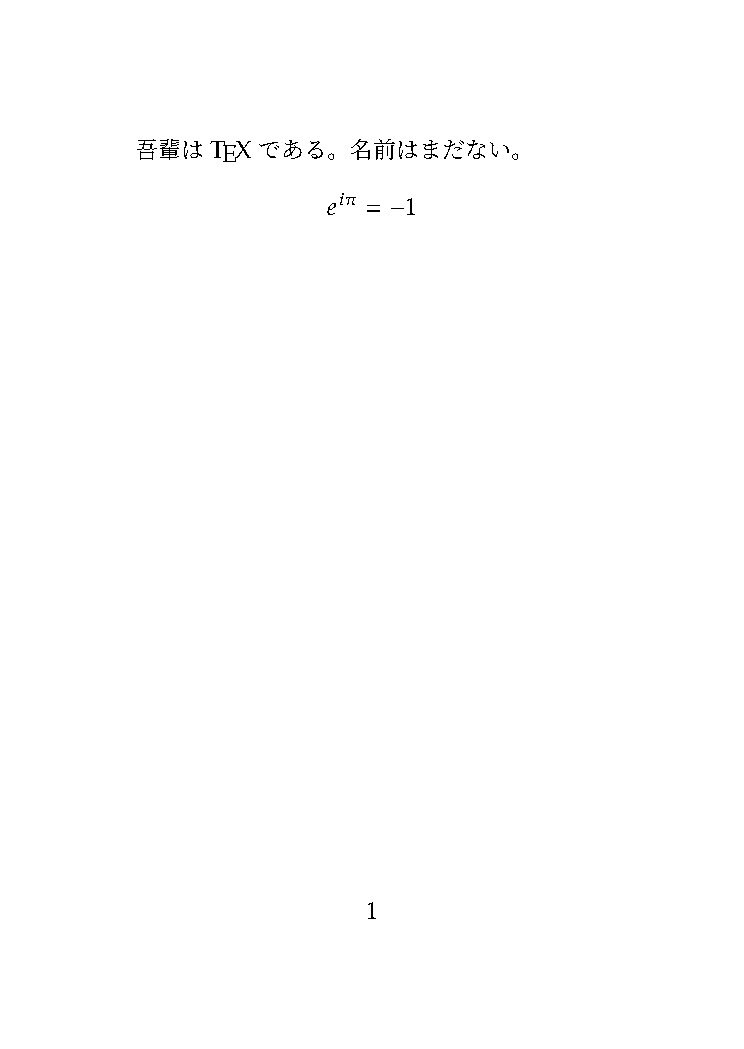
\includegraphics[width=\textwidth]{sample.pdf}}
		\end{column}
	\end{columns}
\end{frame}

\rawstrenable
\begin{frame}[fragile]
	\frametitle{\LaTeX 文書の構造}
	\begin{description}
		\item[{\jruby[g]{命令}{コマンド}}] \texttt{\textbackslash} で始まる、英文字(と和文文字)の列\\
			もしくは \texttt{\textbackslash} のあとに数字か記号ひとつ\\
			\fbox{\texttt{[[|\TeX|]]}} や \fbox{\texttt{[[|\^|]]}} など
			(\jruby[g]{制御語}{コントロールワード}と\jruby[g]{制御文字}{コントロールシンボル})
		\item[環境] \verb+\begin{ナントカ}+ と \verb+\end{ナントカ}+で囲まれたもの
		\item[コメント] \texttt{\%} から行末まではコメント扱い(無視される)
	\end{description}
	
	\begin{block}{特殊な文字}
		以下の文字は特殊文字
		\begin{center}
			\verb+% \ ^ _ ~ { } # & $+
		\end{center}
	\end{block}
\end{frame}
\rawstrdisable

\begin{frame}[fragile]
	\frametitle{\jruby[g]{命令}{コマンド}についての注意}
	\begin{itemize}
		\item \jruby[g]{命令}{コマンド}の引数は \verb+{ }+ で括る
		\item オプショナルな引数は \verb+[ ]+ で括る
	\end{itemize}
	
	\verb+{ }+ はカッコの対応を確認されるが、\\
	{\em\verb+[ ]+ はカッコの対応を確認しない}
	
	例:\\
	\verb+\lstinputlisting[caption=[1]]{foo.tex}+ は\\
	{\em\verb+caption=[1+ だけが \verb+[ ]+ に入っている}判定\\
	→ {\em\verb+[ ]+ に含めたい全体を \verb+{ }+ で括る}と解決\\
	{\footnotesize\verb+\lstinputlisting[{caption=[1]}]{foo.tex}+}
\end{frame}

\begin{frame}[fragile]
	\frametitle{\LaTeX 文書の構造}
	\lstinputlisting{struct.tex}
\end{frame}

\begin{frame}[fragile]
	\frametitle{\LaTeX 文書の構造(ドキュメントクラス)}
	\begin{center}
		\verb+\documentclass[dvipdfmx]{jsarticle}+
	\end{center}
	
	クラスファイルを読み込む→版面構成の定義など\\
	{\footnotesize 実体は ナントカ.cls というテキストファイル}
	
	\begin{block}{主要なクラスファイル}
		\begin{itemize}
			\footnotesize
			\item jsarticle, jsreport, jsbook (新ドキュメントクラス)\\
			\item jlreq(日本語組版処理の要件\footnote{\url{https://www.w3.org/TR/jlreq/ja/}}対応)\\
			\item beamer(スライド用 日本語するには工夫が必要)
			\item jarticle, jreport, jbook(s なし)は\emph{非推奨}
		\end{itemize}
	\end{block}
\end{frame}

\begin{frame}[fragile]
	\frametitle{\LaTeX 文書の構造(ドキュメントクラス)}
	\begin{center}
		\verb+\documentclass[dvipdfmx]{jsarticle}+
	\end{center}
	
	[ ] の中はオプション設定\\
	\bgroup\footnotesize フォントサイズ、見開きの設定など
	\begin{center}
		\verb+\documentclass[12pt,dvipdfmx]{jsarticle}+
	\end{center}
	\egroup
	
	\emph{必ず}使う dvi ウェアをオプションに設定する
	\footnote{dvi 拡張仕様の命令を dvi ファイルに埋め込む必要があるため}
\end{frame}

\begin{frame}[fragile]
	\frametitle{\LaTeX 文書の構造(文書本体)}
	\begin{center}
		\verb+\begin{document}+\\
		$\vdots$\\
		\verb+\end{document}+
	\end{center}
	
	文書本体は \verb+\begin{document}+ と \verb+\end{document}+ の間に書く
	
	打ち込んだ文字がそのまま出力される(特殊文字は除く)
	
	\jruby[g]{命令}{コマンド}を利用できる
\end{frame}

\begin{frame}[fragile]
	\frametitle{文書を書くときの注意}
	\begin{block}{改行の扱い}
		\begin{itemize}
			\item 改行は空白扱い
			\item 和文文字直後の改行は無視(空白にもならない)
			\item 連続した改行→改段落
			\item \verb+%+ は改行文字も含めて、行末まで無視する\\
				→空白は入らない
		\end{itemize}
	\end{block}
	
	メール的なフォーマットで書ける\\
	{\footnotesize 1行が長くなったら改行、改段落は空行}
\end{frame}

\begin{frame}[fragile]
	\frametitle{文書を書くときの注意}
	\begin{block}{\jruby[g]{制御綴}{コントロールシークエンス}や空白の扱い}
		\begin{itemize}
			\item 空白はいくつつなげても 1 つに吸収される
			\item 行頭行末の空白は無視される
			\item \verb*+\ + や \verb+~+ で空白を出力できる(\verb+~+ は行分割されない)
			\item \jruby[g]{制御語}{コントロールワード}直後の空白は
				\emph{\jruby[g]{制御語}{コントロールワード}の区切りでしかない}\\
				→\emph{無視される}
			\item \jruby[g]{制御文字}{コントロールシンボル}直後の空白は\emph{無視されない}
		\end{itemize}
	\end{block}
	
	\bgroup\scriptsize
	\begin{tabular}{lclclcl}
		\verb*+\TeX Live+&→&\TeX Live&\hspace*{3em}&\verb*+\TeX  Live+&→&\TeX  Live\\
		\verb*+\TeX\ Live+&→&\TeX\ Live&&\verb*+{\TeX} Live+&→&{\TeX} Live\\
		\verb*+A \& B+&→&A \& B&&\verb*+A\&B+&→&A\&B
	\end{tabular}
	\egroup
\end{frame}

\begin{frame}
	\frametitle{文書を書くときの注意}
	その他の注意、使える命令、環境は
	\begin{itemize}
		\item \typecommand{texdoc platexsheet-jsclasses}
		\item 美文書作成入門
	\end{itemize}
	を参照
	
	\emph{ググるより先に上を読みましょう}\\
	{\footnotesize ググって出てくる情報は軒並み古くて怪しい
	\footnote{ディスプレイ数式を \texttt{\$\$ 〜 \$\$} で囲んだり、
	\texttt{\textbackslash begin\{eqnarry\}}を使ったり}}
\end{frame}

\begin{frame}[fragile]
	\frametitle{\LaTeX 文書の構造(プリアンブル)}
	\verb+\documentclass+ から \verb+\begin{document}+ の間\\
	→ \emph{プリアンブル (preamble)}
	
	パッケージの読み込み・文書全体の設定をする\\
	{\footnotesize\verb+\usepackage[a4paper]{geometry}+\\
	→ geometry パッケージを、a4paper オプション付きで読み込む}
	
	本文を書くことはできない
	
	逆に、プリアンブルでしか使えないコマンドもある\\
	{\footnotesize \verb+\usepackage+ など}
\end{frame}

\begin{frame}[fragile]
	\frametitle{パッケージとは}
	様々な便利機能を提供\\
	{\footnotesize 他のプログラミング言語で言うところのライブラリ}
	
	実体は、ナントカ.sty というテキストファイル
	
	例: ゆきだるま☃を書きたい!\\
	→ scsnowman パッケージ\\
	→ \verb+\usepackage{scsnowman}+ \\
	→ \verb+\scsnowman[scale=3,hat,arms,buttons]+ \\
	→\scsnowman[scale=3,hat,arms,buttons] 素敵!
\end{frame}

\begin{frame}[fragile]
	\frametitle{パッケージの使い方}
	\begin{enumerate}
		\item 用途からパッケージを探す\\
			{\footnotesize ググるしかない もしくは CTAN でググる
			\footnote{英語なので厳しい; {\tiny ググるを誤用してるのは承知です}}}
		\item プリアンブルで\\\verb+\usepackage[オプション]{パッケージ名}+
		\item 使う
		\item 使い方がわからなくなるので \typecommand{texdoc パッケージ名}
	\end{enumerate}
\end{frame}

\begin{frame}[fragile]
	\frametitle{おすすめプリアンブル}
	\lstinputlisting[basicstyle=\ttfamily\scriptsize]{preamble.tex}
	
	\LaTeX を理解するまでは、これをそのまま使おう
\end{frame}

\begin{frame}[fragile]
	\frametitle{書き方まとめ}
	\lstinputlisting{sample2.tex}
\end{frame}

\frame{\section{エラーへの対処}{\nishikifont 😱美文書 2 章 9 節😱}}

\begin{frame}
	\centering\nishikifont
	\frametitle{\coloremoji{⚠️}ご注意ください\coloremoji{⚠️}}
	\centering\LARGE
	😱😱😱😱😱😱😱😱😱😱
	
	エラー対処が上手かどうかで\\
	作業効率が激変します
	
	😱😱😱😱😱😱😱😱😱😱
\end{frame}

\begin{frame}[fragile]
	\frametitle{エラーに遭遇する}
	\TeX は\emph{プログラミング言語}なので、書き方を間違えるとエラーが出る
	
	\verb+\TEX+ と書いてしまうと……
	
	\pause
	\bgroup\errorfont
	\begin{tabbing}
		! Undefined control sequence.\\
		l.3 \verb+\TEX+\\
	\end{tabbing}
	\egroup
	\pause
	「{\errorfont ?}」と聞かれるので、\keys{X} \keys{Q} \keys{\return} のどれかを押す
\end{frame}

\begin{frame}
	\frametitle{エラーが出たら}
	\begin{description}
		\item[\keys{X}] 処理を中断して終了
		\item[\keys{Q}] 処理を継続、ログは標準出力しない
		\item[\keys{\return}] 処理を継続、再びエラーが出ると止まる
	\end{description}
	
	\keys{\return} を数回連打するのがおすすめ\\
	{\footnotesize 大抵、複数のエラーが混入しているため}\\
	連続して 5 回以上エラーが出てきたら\keys{X}するべし
\end{frame}

\rawstrenable
\begin{frame}[fragile]
	\frametitle{{\errorfont ?} 以外のプロンプトの場合}
	\begin{block}{\fbox{\errorfont Enter file name:}\\
		{\footnotesize \texttt{[[|\usepackage|]]} でパッケージ名を間違えたときに出がち}}
		
		\keys{X}を押して \keys{\return}
	\end{block}
	\vfill
	\begin{block}{\fbox{\errorfont *}\\
		{\footnotesize \texttt{[[|\end{document}|]]} を忘れたときに出がち}}
		\begin{enumerate}
			\item \verb+\stop+ と打って \keys{\return}
			\item \verb+\aaa+(未定義の\jruby[g]{制御綴}{コントロールシークエンス})
				を打って \keys{\return}\\
				→ {\errorfont ?} のプロンプト → \keys{X}
			\item \keys{\ctrl+C}
		\end{enumerate}
	\end{block}
\end{frame}
\rawstrdisable

\begin{frame}
	\frametitle{エラーメッセージの見方}
	
	\bgroup\errorfont
	\begin{tabbing}
		! You can't use `macro parameter character \#' in horizontal mode.\\
		l.3 O-oooooooooo \#\=\\
		                  \>AAAAE-A-A-I-A-U- \\
		?
	\end{tabbing}
	\egroup
	\pause
	
	\begin{tabbing}
	! エラーメッセージ\\
	l. 行数~~~\= \TeX が読み込んだもの\=\\
		\>\>まだ読み込んでいないもの
	\end{tabbing}
	
	エラーが出た行に戻って治せばいいのだが……
\end{frame}

\begin{frame}
	\frametitle{エラーへの対処}
	\begin{block}{大体のエラーの原因}
		\begin{itemize}
			\item \jruby[g]{制御綴}{コントロールシークエンス}の綴りのマチガイ
			\item 環境の閉じ忘れ
			\item ものの不均衡(\texttt{\{ \}}、\texttt{\$ \$}%
				\footnote{\texttt{\$ \$} よりも、\texttt{\textbackslash( \textbackslash)}
				を使うほうが好ましいとされます。(「数式組版」(木枝祐介 ラムダノート
				株式会社\textbf{(2018)}))}、
				\texttt{\textbackslash left \textbackslash right} など)
			\item \jruby[g]{命令}{コマンド}の用法のマチガイ
		\end{itemize}
	\end{block}
	
	エラーが起きた行付近で上がないか確認
	
	\jruby[g]{命令}{コマンド}の用法のマチガイ→\typecommand{texdoc <パッケージ名>} で確認
\end{frame}

\begin{frame}
	\frametitle{対処しにくいエラー}
	\begin{block}{おさらい}
		\LaTeX は \TeX のフォーマット(マクロ体系)\\
		→\emph{\LaTeX レベルのエラーと、\TeX レベルのエラーがある}
	\end{block}
	起きたエラーによっては、原因が特定しにくい\\
	{\footnotesize 例: {\errorfont ! Missing number, treated as zero.}}
	
	\pause
	処理中に外部ファイルを読み込むこともある\\
	→行番号が、\emph{どのファイルの行番号かわからなくなる}
\end{frame}

\begin{frame}[fragile]
	\frametitle{エラーを起こさないために}
	\begin{itemize}
		\item タイプセットを細かく行う
		\item 開いた環境はすぐ閉じる
		\item 全角空白「 」を使わない\\
			{\footnotesize 段落頭の字下げは \verb+\parindent+ で設定\\
			\tiny 欧文クラスで、一番最初のパラグラフを字下げしたい場合 → indentfirst パッケージ}
		\item \verb+\verb+ 命令もなるべく避ける\\
			{\footnotesize \jruby[g]{命令}{コマンド}の引数にあるとエラー(\verb+\verb+ の呪い)}
	\end{itemize}
	\pause
	それでも意味不明なエラーが起きる
\end{frame}

\begin{frame}[fragile]
	\frametitle{パッケージの衝突}
	\lstinputlisting[basicstyle=\ttfamily\scriptsize]{error.tex}
	\vspace{-1ex}\centeralign{↓}\vspace{-1ex}
	\bgroup\errorfont\scriptsize
	\begin{tabbing}
		! LaTeX Error: \=Command \verb+\iint+ already defined.\\
		\>Or name \verb+\end+... illegal, see p.192 of the manual.\\
		l.645 ...d\verb+{\iint}{\DOTSI\protect\MultiIntegral{2}}+\\
	\end{tabbing}
	\egroup \pause
	mathabx と ymasth が同じ\jruby[g]{命令}{コマンド}を定義→エラー
\end{frame}

\begin{frame}
	\frametitle{衝突の回避}
	パッケージを読み込む順番を変えたら誤魔化せる場合も\\
	→ 読み込む順番を変えてみる\\
	→ どうしようもなければ諦める
	
	パッケージが日本語対応してなくてエラーが起きる場合も\\
	→ (u)p\LaTeX なら plautopatch パッケージ
	\footnote{\url{https://aminophen.github.io/slide/hytexconf18.pdf}}を試す\\
	→ \LuaLaTeX なら日本語非対応の問題はおこりにくい
\end{frame}

\begin{frame}
	\frametitle{エラーが解消できなくてどうしようもないときは}
	とりあえずエラーメッセージでググってみる\\
	{\tiny これで解決できたら苦労しないんだよなぁ わかりにくいエラーメッセージが嫌ならば、\SATySFi ……?}
	
	わからなければ詳しい人に聞く\\
	{\footnotesize TeX Forum\footnote{\url{https://oku.edu.mie-u.ac.jp/tex/}} で質問\\
	Twitter でつぶやくのも実は有用}
	
	実はバグを踏んでいる可能性も
\end{frame}

\begin{frame}[fragile]
	\frametitle{わかりにくいエラー①}
	
	\verb+[a] 真鍋 \\ [b] いつき+\\
	→{\errorfont ! Missing number, treated as zero.}
	
	\verb+\\+(強制改行)命令は、実はオプション引数をもつ\\
	\hspace*{1em}→\verb+\\[<長さ>]+
	
	\verb+\\{}+ のように \verb+{}+で区切ると解決
	
	\bgroup\footnotesize
	\begin{tabbing}
		\verb+[a] 真鍋 \\{} [b] いつき+\\
		→\=[a] 真鍋 \\{} \> [b] いつき
	\end{tabbing}
	\egroup
\end{frame}

\rawstrenable
\begin{frame}[fragile]
	\frametitle{わかりにくいエラー②}
	
	\verb+\section{$\overrightarrow{\mbox{ぶーん}}$}+\\
	→{\errorfont ! Illegal parameter number in definition of \verb+\reserved@a+.}
	
	エラーが起きる原因→\coloremoji{🤮}
	\footnote{{\ttfamily[[|\section|]]} の引数は動くので、脆弱な 
	{\ttfamily[[|\overrightarrow|]]} は保護しなければならない}
	
	\verb+\section+ や \verb+\caption+ で変なエラーが出たら、\\
	引数に入ってるヤバそうな\jruby[g]{命令}{コマンド}に \verb+\protect+ を前置
	
	{\footnotesize\verb+\section{$\protect\overrightarrow{\mbox{ぶーん}}$}+\\
	→ $\protect\overrightarrow{\mbox{ぶーん}}$}
\end{frame}
\rawstrdisable

\frame{\section{\TeX のディレクトリ構成} {\nishikifont ☃美文書 付録 B 3 節☃}}

\begin{frame}
	\frametitle{TEXMF ツリー}
	\TeX 関連ファイルを入れるディレクトリ構成\\
	{\footnotesize TEXMF ← \TeX + \MF\footnote{\MF は Knuth が作ったフォント記述言語}}
	
	複数の TEXMF ツリーを使い分けるのが主流\\
	\emph{多重 TEXMF ツリー}
	
	確認方法: \typecommand{kpsewhich -var-value TEXMF}
\end{frame}

\begin{frame}
	\frametitle{多重 TEXMF ツリーの利点}
	ディストリビューションが用意したファイルと、自分がインストールしたファイルを分離できる
	
	ディストリビューションを更新しても、自分のインストールしたファイルは削除されない
	
	\begin{tabbing}
	\hspace*{3\zw}\=\kill
	ディストリビューションが用意したファイル\\
		\>{→\scriptsize\typecommand{kpsewhich -var-value TEXMFDIST}}\\
	自分がインストールするファイル\\
		\>{→\scriptsize\typecommand{kpsewhich -var-value TEXMFLOCAL}}\hspace{1\zw}\={\scriptsize 全ユーザーが使える}\\
		\>{→\scriptsize\typecommand{kpsewhich -var-value TEXMFHOME}}\>{\scriptsize そのユーザーが使える}
	\end{tabbing}
\end{frame}

\begin{frame}
	\frametitle{kpathsea ライブラリ と \aruby{ls-R}{ファイル一覧}}
	\begin{block}{kpathsea ライブラリ}
		TEXMF ツリーからファイルを検索する\\
		{\footnotesize Karl Berry 氏によって作られた path searching}
		
		例: \typecommand{kpsehwhich hmtrump.sty}\\
		{\scriptsize →\texttt{/usr/local/texlive/texmf-local/tex/latex/local/hmtrump.sty}}
	\end{block}
	
	TEXMF ツリーに作られた \aruby{ls-R}{ファイル一覧} を見て検索する\\
	TEXMF ツリーに変更 → \aruby{ls-R}{ファイル一覧} を更新する必要
	\footnote{ls-R を使わない運用方法もあるらしいですが、やったことがないのでわかりません}\\
	\typecommand{sudo mktexlsr}
\end{frame}

\begin{frame}
	\frametitle{パッケージをインストールする}
	ディストリビューションに含まれないパッケージを使いたい\\
	→自分で TEXMF ツリー \textbf{(TEXMFLOCAL)} に入れる必要\\
	{\footnotesize 作業ディレクトリに置いてもよいけれども}
	
	正しい場所に入れなければ正常に使えない
	\footnote{拡張子に応じて、検索するディレクトリを決め打ってるため}
\end{frame}

\begin{frame}
	\frametitle{TEXMF ツリーの構造}
	TEXMFLOCAL\footnote{{\TeX} Live on UNIX の標準では \texttt{/usr/local/texlive/texmf-local}}
	の構造を覗いてみる
	\footnote{\href{https://texwiki.texjp.org/?TeX\%20\%E3\%81\%AE\%E3\%83\%87\%E3\%82\%A3\%E3\%83\%AC\%E3\%82\%AF\%E3\%83\%88\%E3\%83\%AA\%E6\%A7\%8B\%E6\%88\%90}
	{https://texwiki.texjp.org/?TeX\%20のディレクトリ構成}参照}\\
	\typecommand{tree -d -L 2 /usr/local/texlive/texmf-local}
	
	\begin{columns}
		\begin{column}{0.6\textwidth}
			ファイルの種類ごとに分類
			\begin{description}
				\small
				\item[doc] ドキュメント(説明書)
				\item[tex] パッケージの本体など
				\item[font] フォント関連
			\end{description}
			さらにサブディレクトリで分類\\
			そのなかでパッケージごとに分類
		\end{column}
		\begin{column}{0.35\textwidth}
			\tiny\ttfamily
			/usr/local/texlive/texmf-local\\
			├── doc\\
			│   ├── fonts\\
			│   ├── latex\\
			│   └── lualatex\\
			├── source\\
			│   └── latex\\
			├── tex\\
			│   ├── latex\\
			│   ├── lualatex\\
			│   └── plain\\
			├── texdoc\\
			├── tlpkg\\
			└── web2c
		\end{column}
	\end{columns}
\end{frame}

\begin{frame}
	\frametitle{パッケージをインストールする場所}
	前述の通り、分類して TEXMFLOCAL に配置
	
	まずはパッケージドキュメントを確認
	
	\begin{block}{ドキュメントに記載がない場合: あまり失敗しない方法}
		以下にディレクトリを掘ってファイルを配置
		\begin{itemize}
			\small
			\item ドキュメント→ \texttt{\$TEXMFLOCAL/doc/latex/<pkgname>}
			\item *.dtx, *.doc→ \texttt{\$TEXMFLOCAL/source/latex/<pkgname>}
			\item その他→ \texttt{\$TEXMFLOCAL/tex/latex/<pkgname>}
		\end{itemize}
	\end{block}
	
	フォント関連などはもっと複雑
\end{frame}

\begin{frame}
	\frametitle{参考文献}
	\emph{とりあえず美文書は読んでください}
	
	\begin{block}{もっと詳しく知りたい場合}
		\begin{itemize}
			\item {\TeX} Wiki\\\url{https://texwiki.texjp.org}
			\item Acetaminophen'{\kern-0.7em}s diary\\\url{http://acetaminophen.hatenablog.com}
		\end{itemize}
	\end{block}
	
	\bgroup\footnotesize
	\begin{block}{以下のブログは、もっと沼にハマりたい人向け}
		\begin{itemize}
			\item ラングラグー\\\url{https://blog.wtsnjp.com}
			\item マクロツイーター\\\url{https://zrbabbler.hatenablog.com}
		\end{itemize}
	\end{block}
	\egroup
\end{frame}
\end{document}
